\chapter{07/12/16 - Legge di Gruppo sulla cubica e Gruppo dei Divisori}
\justify

\section{Legge di gruppo sulla cubica}
Abbiamo già visto che con la proiezione al quoziente $\pi : \mathbb{C} \rightarrow T$ il toro eredita la struttura di gruppo additivo da $\mathbb{C}$.
Vogliamo vedere adesso chi è la legge di gruppo sulla cubica $\widetilde{E}$.
Considero la mappa di Weierstrass: $T\rightarrow \widetilde{E}$ che manda $z \rightarrow (\wp(z):\wp'(z):1)$. Mi chiedo chi sia l'immagine di $z_1 + z_2$.

\begin{teorema}
$$\wp(z_1+z_2)=\frac{a^2}{4}-\wp(z_1)-\wp(z_2)$$
con $a=\displaystyle{\frac{\wp'(z_2)-\wp'(z_1)}{\wp(z_2)-\wp(z_1)}}$.
\end{teorema}

\begin{proof}
Cerco dei coefficienti $a,b$ tali che $\wp'(z)=a\wp(z)+b$ si annulli in $z_1$ e $z_2$.
Risolvendo ottengo:

\begin{displaymath}
  \left\{
    \begin{array}{l}
      a = \frac{\wp'(z_2) - \wp'(z_1)}{\wp(z_2) - \wp(z_1)} \\
      b = - \frac{\wp'(z_2) \wp(z_1) - \wp'(z_1) \wp(z_2)}{\wp(z_2) - \wp(z_1)} \\
    \end{array}
  \right.
\end{displaymath}

Supponiamo $\wp(z_2) \neq \wp(z_1)$, altrimenti ho due casi: $z_2 \equiv z_1$, che tratterò alla fine, e $z_2 \equiv -z_1$.
In quest'ultimo caso la formula di addizione perde di senso, perché $\wp$ ha un polo in zero.


Considero la funzione $\wp'(z) - a \wp(z) - b$: è una funzione ellittica.

Inoltre, pensata nei complessi, ha poli solo nei punti del reticolo $L$, quindi pensata sul toro ha un polo solo in zero, ed è di ordine 3.
Allora ha 3 zeri, di cui sicuramente due sono $z_1$ e $z_2$. Chiamo $z_3$ l'altro zero.

Un teorema che abbiamo visto (T3) assicura che per le funzioni ellittiche $$ \sum_\text{zeri} z_i - \sum_\text{poli} w_i \equiv 0$$.

Nel nostro caso $z_1 + z_2 + z_3 - (0+0+0) \equiv 0$, da cui $z_3 \equiv - z_1 - z_2$.

Imponendo ora che $\wp'(z) - a \wp(z) - b$ si annulli in $ -z_1 - z_2 $, ottengo:
$$ \wp'(-z_1-z_2) - a \wp(-z_1-z_2) - b = 0 $$
Da questo e dalla parità/disparità di $ \wp, \wp' $ segue:
$$ - \wp'(z_1+z_2) = a \wp(z_1+z_2) + b $$
Ora ricordo che: $$ - \wp'(z_1+z_2)^2 = 4 \wp(z_1+z_2)^3 - g_2 \wp(z_1+z_2) - g_3 $$
Mettendo a sistema queste due equazioni si ottiene:
$$4 \wp(z)^3 -a^2 \wp(z)^2 - (2ab+g_2) \wp(z) - g_3 - b^2=0$$
$$\wp(z)^3 -\frac{a^2}{4} \wp(z)^2 - \frac{(2ab+g_2)}{4} \wp(z) - \frac{(g_3 - b^2)}{4}=0$$
nei punti $z_1, z_2, z_3$.

Ovvero, pensandolo come un polinomio in $\wp(z)$, ha come radici $\wp(z_1), \wp(z_2), \wp(z_3)$.
Per le relazioni radici-coefficienti so che: $\frac{a^2}{4} = \wp(z_1) + \wp(z_2) + \wp(z_3)$.

$$\wp(z_1+z_2) = \frac{a^2}{4} - \wp(z_1) - \wp(z_2)$$
che è la formula di addizione che stavamo cercando.


Si può dimostrare che vale per ogni $z_1, z_2$, anche uguali (purché diversi da $0$), si tratta di fare
$$ \lim_{z_1 \rightarrow z_2} \frac{a^2}{4} - \wp(z_1) - \wp(z_2)$$ con De L'Hopital. 
\end{proof}


Notiamo con stupore che è un espressione razionale, cosa che a priori non era ovvia.
In modo analogo si può ricavare una formula di addizione per $\wp'$.

\begin{osservazione}
Ricordando che la mappa di Weierstrass pensata in modo affine è $z \rightarrow (\wp(z),\wp'(z))$, ho quindi dimostrato che la mappa di Weirstrass induce la seguente struttura di gruppo su $E$:
$(x_1,y_1) + (x_2,y_2) = (x_3,y_3)$ con

\begin{displaymath}
  \left\{
    \begin{array}{l}
      x_3 = \frac{(y_2-y_1)^2}{a(x_2-x_1)} - x_1 - x_2 \\
      y_3 = ax_3 + b \\
    \end{array}
  \right.
\end{displaymath}
\end{osservazione}

\begin{osservazione}: le traslazioni sono automorfismi della cubica. Sono mappe dalla curva in sé non banali e razionali.
L'inversa di $\tau_z$ è $\tau_{-z}$
\end{osservazione}


\section{Legge di gruppo geometrica sulla cubica}
Definisco $P_1 * P_2 = P_3$ come in figura.
\begin{center}
  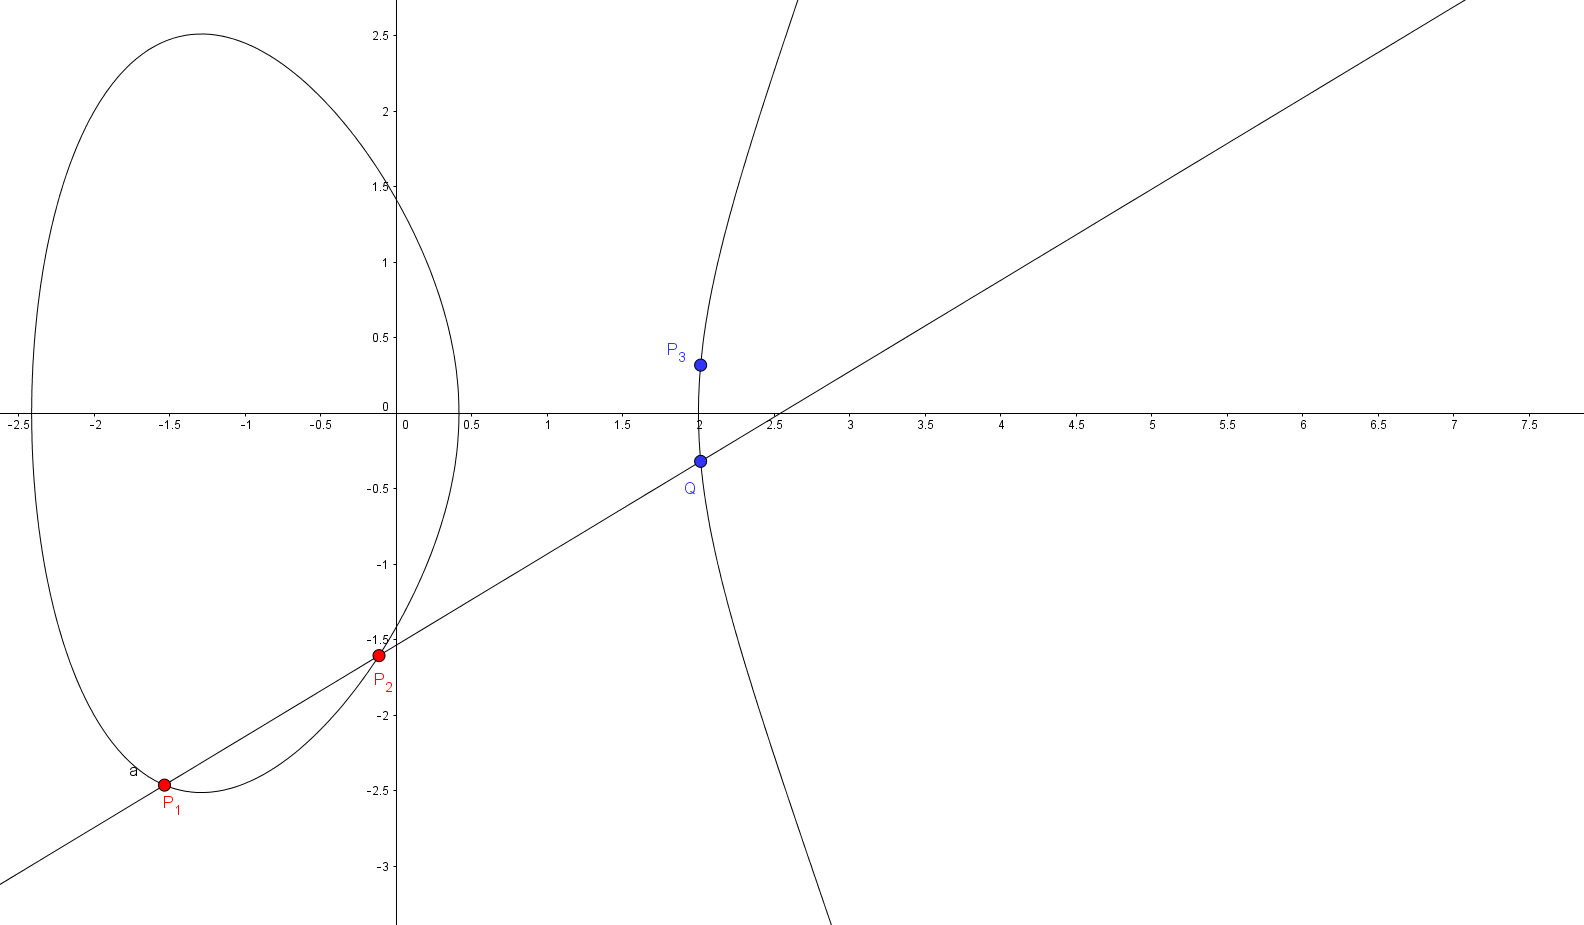
\includegraphics[width=0.8\linewidth]{lezione-161207-fig1}
\end{center}
%\textbf{Allegare figura! Balbo, ci ho provato ma non ci sono riuscita..}

%\begin{figure}
%	\centering
	%	\includegraphics{C:/Users/Clara/Desktop/Università/3 anno/Corsi/Zannier lez15/Figura lezione 071216.png}
%	\label{fig:Figura lezione 071216}
%\end{figure}


\begin{proposizione}
La funzione $*$ appena definita è una legge di gruppo commutativa.
\end{proposizione}
\begin{proof}
La commutatività è ovvia.
L'elemento neutro è il punto all'infinito (si vede per ragioni geometriche).
L'inverso di $P$ è $-P$.
Il vero osso duro è l'associatività, che in questo corso non dimostriamo.
\end{proof}

\begin{osservazione}
Se sappiamo che la cubica proviene da un toro, possiamo dire che la legge di gruppo $*$ proviene dal $+$ del toro (sotto quali ipotesi valgono sti sollevamenti mi sfugge). In questo modo anche l'associatività diventa ovvia.
\end{osservazione}

\section{Equivalenza lineare tra divisori (sulle cubiche)}

\begin{definizione}
Definiamo il gruppo dei divisori sulla cubica $\Div(\widetilde{E})$ come il gruppo abeliano libero generato dai punti della cubica. Per gli analisti, me compresa, significa che è l'insieme delle combinazioni formali finite del tipo $$\sum_{P \in \widetilde{E}} \alpha_P(P)$$,
con $\alpha_P \in \mathbb{Z}$.
Sempre per gli analisti: coraggio ragazzi, mancano poche lezioni!
RIP per questi commenti che verranno cancellati da Balbo, stima per lui se invece li lascia.
% Vabbè li lasciamo anche se sarebbe meglio di no. Balbo
Attenzione: anche la stringa vuota ($\alpha_P=0$ $\forall P$) è un elemento, in particolare è l'elemento neutro.
Equivalentemente posso pensarle come le funzioni dalla cubica in $\mathbb{Z}$ a supporto finito.
\end{definizione}

\begin{definizione}
Si definisce grado di un divisore il numero $$\sum \alpha_P \in \mathbb{Z}$$.
\end{definizione} 

\begin{osservazione}Il grado è un omomorfismo di gruppi $\deg: \Div(\widetilde{E}) \rightarrow \mathbb{Z}$.
\end{osservazione}


\begin{definizione}
Si definisce gruppo dei divisori di grado zero sulla cubica $\Div^0(\widetilde{E}) := \Ker(\deg)$.
\end{definizione}

\begin{definizione}
Per questa definizione supponiamo di sapere che la cubica viene da un toro.
Considero una funzione $f$ razionale non nulla su $\widetilde{E}$, cioè $f \in \mathbb{C}(\wp(z),\wp'(z))$. So che ha finiti zeri e finiti poli.
Si definisce: $\div(f) = \sum_{P\in T} \ord_P(f) \cdot (P) \in \Div(\widetilde(E))$.
L'insieme di tutti i possibili $\div(f)$ si chiama insieme dei divisori principali.
\end{definizione}

Un teorema che abbiamo visto (T2 sulle superfici di riemann compatte) garantisce che $\div(f) \in \Div^0(\widetilde{E})$
Inoltre $\{\div(f)\}$ è un sottogruppo di $\Div^0(\widetilde{E})$ (le verifiche sono banali).

C'è dunque un omomorfismo (non surgettivo) tra il gruppo moltiplicativo delle funzioni razionali non nulle su $\widetilde{E}$ e i divisori di grado zero.
$\varrho: \mathbb{C}(\widetilde(E))^* \rightarrow \Div^0(\widetilde{E})$. Infatti $\div(fg)=\div(f)+\div(g)$.

\begin{proposizione}
$\Ker(\varrho) = \{\text{le funzioni costanti diverse da zero}\}$
\end{proposizione}
\begin{proof}
Un'inclusione ($\supseteq$) è banale, per l'altra possiamo osservare che se $\varrho(g)$ va nell'elemento
neutro di $\Div^0(\widetilde{E})$ (la stringa vuota), allora essa non ha né poli né zeri (neanche all'infinito), ma allora è necessariamente costante.
\end{proof}

\begin{osservazione}
Quindi ho una successione esatta che comincia così:
$$0 \rightarrow \mathbb{C}^* \rightarrow \mathbb{C}^*(\widetilde{E}^*) \rightarrow \Div^0(\widetilde{E})$$
\end{osservazione}


\section{Divisori in un caso più semplice: $\mathbb{P}_1$}
$\mathbb{C}(\mathbb{P}_1) = \mathbb{C}(t)$ con $t$ che è la funzione coordinata $t(x_1, x_0)=\frac{x_1}{x_0}$.
Ha un polo nel punto all'infinito, cioè in $(1:0)$.

\begin{proposizione}
Ogni divisore di grado $0$ è il divisore di una funzione (nel caso di $\mathbb{P}_1$! Per $\widetilde(E)$ è falso.)
\end{proposizione}
\begin{proof}
Possiamo supporre che $\infty$ non compaia nel divisore di grado $0$ (infatti, se per caso ci compare con coefficiente $n$,
sarà sufficiente sottrarre alla fine una funzione che ha un solo polo di ordine $n$ all'infinito).
Allora (col piccolo abuso di identificare $\mathbb{P}_1 \backslash \infty$ con $\mathbb{C}$)
questo divisore sarà $\sum m_i (\alpha_i)$ con $m_i \in \mathbb{Z}$ e $\alpha_i \in \mathbb{C}$, e so che $\sum m_i=0$.
Calo dal cielo $\prod(t-\alpha_i)^m_i$, e si vede facilmente che risolve.
\end{proof}


\section{Torniamo sulle cubiche: il gruppo di Picard}
In generale possiamo definire:

\begin{definizione}
$\Pic^0(\widetilde{E}) := \frac{\Div^0(\widetilde{E})}{\text{divisori principali}}$
\end{definizione}

\begin{osservazione}
Ho quindi la successione esatta:
$$0 \rightarrow \mathbb{C}^* \rightarrow \mathbb{C}^*(\widetilde{E}^*) \rightarrow \Div^0(\widetilde{E})\rightarrow \Pic^0(\widetilde{E})\rightarrow 0$$
\end{osservazione}

Nel caso visto prima di $\mathbb{P}_1$, già $\Pic^0(\mathbb{P}_1)=0$

\notamargine{
Avere il $\Pic=0$ è imparentato in qualche modo con l'essere UFD. Ad esempio $\mathbb{Z}(i)$ ha $\Pic=0$. Nel caso del $\mathbb{P}_1$, il fatto che il suo $\Pic$ sia nullo è dunque legato alla fattorizzazione unica dei polinomi.
}

\section{Vogliamo ora studiare il Pic di una curva ellittica}

Considero $\sigma : \widetilde(E) \rightarrow \Div^0(\widetilde(E))$ tale che $\sigma(P)=(P)-(0)$
Considero un divisore di grado $0$ su $E$. Sarà della forma $d = \sum\alpha_P\cdot(P)$.
Poiché $\sum \alpha_P=0$, lo posso scrivere come $\sum\alpha_p \sigma(P)$.

\begin{definizione}
Equivalenza lineare tra divisori. Si dice che $d_1 \sim d_2$ se $d_1-d_2$ è un divisore principale. Attenzione! Non tutti i divisori di grado zero sono principali.
\end{definizione}

\begin{teorema}
Ogni divisore di grado zero è linearmente equivalente ad un $\sigma(P)$.
\end{teorema}

Alla dimostrazione premettiamo alcuni lemmi. 
\begin{lemma}
$(R) + (-R) \sim 2(0)$
\end{lemma}
\begin{proof}
Sia $R$ è il punto di $\widetilde(E)$ associato al punto $z_0 \in T$.
Dimostro ora che $(R)+(-R)-2(0)$ è un divisore principale, da cui $(R)+(-R)-2(0) \sim \varnothing$ da cui la tesi.
Ma considerando la funzione $\wp(z)-\wp(z_0)$ si vede che ha divisore $(R)+(-R)-2(0)$ (polo doppio in $0$, zeri semplici in $R,-R$), da cui la tesi.
\end{proof}


\begin{lemma}
$\sigma(P)+\sigma(Q) \sim \sigma (P+Q)$
\end{lemma}


\begin{proof}
La tesi equivale a:
$$(P)-(0)+(Q)-(0) \sim (P+Q)-(0)$$
$$(P)+(Q)\sim (P+Q)+(0)$$
Attenzione: si intende che il $+$ fuori dalle parentesi è la legge di gruppo che abbiamo visto nel Teorema \ref{leggedigruppo}, mentre il $+$ fuori dalla parentesi è il $+$ formale dei divisori.
Considero la funzione $h(z) = \wp'(z) - a \wp(z) - b$ con a e b definiti come nel Teorema \ref{leggedigruppo}. Abbiamo già visto che ha un polo di ordine $3$ nell'origine e tre zeri semplici in $P, Q, -P-Q$. Quindi $$\Div(h)=(P)+(Q)+(-P-Q)-3(0) \sim \varnothing$$
Utilizzo ora il lemma \ref{lemma_equiv_lin}, e ottengo che:
$$(P)+(Q)+2(0)-(P+Q)-3(0) \sim \varnothing$$
$$(P)+(Q) \sim (P+Q)-(0)$$
\end{proof}

\begin{proof}[Dimostrazione del Teorema]
Considero un qualsiasi divisore $d$ di grado $0$.
$$d=\sum a_i (P_i)$$
per $i=1,...,n$. So che $\sum a_i=0$. Allora:
$$d=\sum a_i (P_i)-\sum a_i (0)=\sum a_i ((P_i)-(0))=\sum a_i (\sigma(P_i))$$
Ma adesso estendendo banalmente il lemma \ref{lemma_equiv_lin2} dalle somme alle combinazioni lineari, ottengo che:
$$d=\sum a_i (\sigma(P_i))=\sigma(\sum a_i P_i)$$
da cui la tesi.
\end{proof}